\chapter{Vortex connections across topological interfaces}\label{chap: spin-2}
In this chapter, we both analytically and numerically investigate the physics
of topological defects when connected across topological interfaces in spin-2
Bose-Einstein condensates.
We demonstrate that a particularly rich phenomenology of topological defects
at the coherent
interface between regions of different broken symmetries can be realised in
spin-2 Bose-Einstein condensates.
In particular, we propose that an interface between uniaxial and biaxial nematic
phases exhibiting continuous and discrete order-parameter symmetry,
respectively, can be realised using existing experimental techniques.
We construct spinor wave functions that represent topological defects connecting
across the interface.
By numerical energy relaxation as well as simulations of dynamics, we
characterise the emergence of non-trivial defect core structures.
We further demonstrate the emergence of composite vortex-core structures and
continuous connection of fractional vortices representing non-Abelian charges in
interfaces involving the cyclic and ferromagnetic phases, which could be
realised through manipulation of the inter-atomic interactions.
Our results suggest the spin-2 Bose-Einstein condensates as experimentally
accessible test beds for interface physics with all combinations of continuous
and discrete symmetries, as well as phases supporting non-Abelian defects.

\section{Introduction to topological interfaces}
When topologically distinct phases, described by different order parameters,
coexist in a continuous and coherent ordered medium, a topological interface
must form at the phase boundary, where the different broken symmetries connect
smoothly.
Such interfaces are ubiquitous across many areas of physics, from the
\(A\)--\(B\) phase boundary in superfluid
helium~\cite{Salomaa1987, Volovik2009, Finne2006}, to appearing as the
termination points of cosmic strings in theories of the early
universe~\cite{Kibble1976, Vilenkin1994}, and even in brane-inflation
models in superstring theory~\cite{Dvali1999, Sarangi2002}.
They may also play an important role for superconducting materials in
solid-state physics~\cite{Bert2011}.
The different order-parameter symmetries imply that the bulk medium on either
side of the interface supports different families of topological defects and
textures, which therefore cannot cross the interface unchanged, but must either
terminate, or connect continuously and non-trivially to an object representing
the different topology on the other side.
Due to the ubiquitous nature of topological interfaces, their study in
controlled experiments becomes of general importance, inspiring the use of
laboratory systems as emulators for interface physics in contexts otherwise not
amenable to experimental observations, for example the simulation of
brane-collision processes using superfluid \(^3\)He~\cite{Bradley2007}.

Topological-interface physics becomes especially intriguing when the medium on
either or both sides of the interface exhibits point-group order-parameter
symmetry~\cite{Xiao2022}, leading to the existence of non-Abelian defects,
whose charges depend on the presence of other defects in the system and whose
dynamics is highly constrained~\cite{Poenaru1977,Mermin1979,Kobayashi2009}.
Such fully discrete order-parameters symmetries readily arise in particular
phases of spin-2 and -3 Bose-Einstein condensates
(BECs)~\cite{Barnett2006,Barnett2007,Semenoff2007,Makela2007,Yip2007,
    Kobayashi2009,Borgh2016b,Xiao2022}, which have consequently been proposed, e.g.,
as candidates for quantum-computation applications~\cite{Mawson2019} and for
realisation of non-Abelian quantum turbulence~\cite{Mawson2015}.
Spinor BECs~\cite{Kawaguchi2012,StamperKurn2013} are constructed in all-optical
traps such that the internal spin-degrees of freedom are not frozen out by
strong magnetic fields~\cite{StamperKurn1998} and provide an ideal
testing ground for investigating interface
physics~\cite{Borgh2012,Borgh2013,Borgh2014}.
Their rich phase diagrams~\cite{Kawaguchi2012} exhibit a rich variety of
phases with different order-parameter symmetries, supporting radically different
families of topological defects, such as singular
vortices~\cite{Yip1999,Isoshima2002,
    Zhou2003,Ji2008,Takahashi2009,Lovegrove2012,Weiss2019,Xiao2021}, including
vortices carrying fractional circulation~\cite{Leonhardt2000,Ji2008,Seo2015,
    Semenoff2007,Borgh2016b,Xiao2022}, and non-singular
textures~\cite{MizushimaPRL2002, MizushimaPRA2002,
    Martikainen2002,Choi2012,Lovegrove2014},
monopoles~\cite{Pietila2009,Ollikainen2017,Ruostekoski2003,Ray2014,Ray2015,
    Mithun2022}, and even Skyrmions~\cite{Tiurev2018,Lee2018} and
knots~\cite{Hall2016}.

With spin-2 BECs being experimentally readily realisable~\cite{Schmaljohann2004}
and  experimental techniques for controlled creation of vortices with internal
point-group symmetries having recently been developed~\cite{Xiao2022}, these
systems are poised as immediate candidates for the realisation of topological
interfaces with non-Abelian defect physics. Here we analytically construct spinor
wave functions representing continuous defect connections across all
permutations of topological interfaces between the different ground-state
phases of spin-2 BECs and demonstrate their energy relaxation by numerical
simulation for illustrative examples. We have previously suggested that
topological interface could be realised in spin-1 BECs through the spatial
engineering of induced Zeeman shifts~\cite{Borgh2014} (which can also control
the defect-core symmetry properties~\cite{Borgh2016a,Underwood2020}) or, less
straightforwardly, using optical or microwave Feshbach resonances to manipulate
atomic scattering lengths~\cite{Borgh2012,Borgh2013}. Here we show how the
former technique readily lends itself to the formation of a topological
interface between uniaxial (UN) and biaxial nematic (BN) phases with commonly
used atomic species such as \({87}\)Rb. We construct solutions corresponding to
connecting singly quantized and spin vortices, as well as terminating vortices.
\textcolor{red}{[Something more here]}

\section{Interface crossing solutions in a spin-2 BEC}
As discussed in Chapter~\ref{chap: ground-states}, the spin-2 BEC gives rise to
three ground state phases in the absence of a magnetic field: Ferromagnetic,
nematic, and cyclic.
In addition to these states, additional steady-state solutions that arise in
the presence of Zeeman shifts~\cite{Kawaguchi2012}.
Here, we derive a subset of the stationary solutions that offer interpolating
solutions between different ground states.

Stationary solutions of the spin-2 GPEs are obtained by substituting
\(\psi_m = \sqrt{n}\zeta_m e^{-i\mu t/\hbar}\) into
Eqs.~\eqref{eq: spin-2-GPEs-pm2}-\eqref{eq: spin-2-GPEs-0}.
Ignoring the kinetic energy term and taking \(V(\vb{r}) = 0\), this results
in
\begin{align}
    \mu\zeta_2    & = \left(-2p + 4q + c_0n +2c_1nf_z\right)\zeta_2
    + c_1nf_-\zeta_1 + \frac{c_2}{\sqrt{5}}na_{00}\zeta^*_{-2},            \\
    \mu\zeta_1    & = \left(-p + q + c_0n +c_1nf_z\right)\zeta_1
    + c_1\left(\frac{\sqrt{6}}{2}nf_-\zeta_0 +nf_+\zeta_2\right)
    - \frac{c_2}{\sqrt{5}}na_{00}\zeta^*_{-1},                             \\
    \mu\zeta_0    & = c_0n\zeta_0 + \frac{\sqrt{6}}{2}c_1\left(nf_+\zeta_1
    + nf_-\zeta_{-1}\right) + \frac{c_2}{\sqrt{5}}na_{00}\zeta_0^*,        \\
    \mu\zeta_{-1} & = \left(p + q + c_0n - c_1nf_z\right)\zeta_{-1}
    + c_1\left(\frac{\sqrt{6}}{2}nf_+\zeta_0 +nf_-\zeta_{-2}\right)
    - \frac{c_2}{\sqrt{5}}na_{00}\zeta^*_{1},                              \\
    \mu\zeta_{-2} & = \left(2p + 4q + c_0n - 2c_1nf_z\right)\zeta_{-2}
    + c_1nf_+\zeta_{-1} + \frac{c_2}{\sqrt{5}}na_{00}\zeta^*_{2}.          \\
\end{align}

We can choose the overall phase such that \(\zeta_0\) is real.
In addition, since the system is assumed to be symmetric about the \(z\)-axis,
we can let \(f_y=0\) without loss of generality.
\textcolor{red}{Need to convince myself on this last assumption.}
We consider the specific case where the transverse magnetisation is zero
\(f_{\pm} = 0\), which is valid for \(q < 0\)
Assuming the above, the stationary equations can be transformed into the
following simplified set of equations:
\begin{align}
    0 & = (-2p + 4q + c_0n + 2c_1nf_z - \mu)\zeta_2
    + \frac{c_2}{\sqrt{5}}na_{00}\zeta^*_{-2},
    \label{eq: spin-2-stationary-zeta2}                                 \\
    0 & = (2p + 4q + c_0n - 2c_1nf_z - \mu)\zeta_{-2}
    + \frac{c_2}{\sqrt{5}}na^*_{00}\zeta_{2},
    \label{eq: spin-2-stationary-zetam2}                                \\
    0 & = (-p + q + c_0n + c_1nf_z - \mu)\zeta_1
    + \frac{c_2}{\sqrt{5}}na_{00}\zeta^*_{-1},
    \label{eq: spin-2-stationary-zeta1}                                 \\
    0 & = (p + q + c_0n - c_1nf_z - \mu)\zeta_{-1}
    + \frac{c_2}{\sqrt{5}}na^*_{00}\zeta_1,
    \label{eq: spin-2-stationary-zetam1}                                \\
    0 & = \left(c_0n + \frac{c_2}{\sqrt{5}}na_{00} - \mu\right)\zeta_0.
    \label{eq: spin-2-stationary-zeta0}
\end{align}

Noting that the above equations are decoupled in three parts, we can construct
the following matrix equations relating to
Eqs.~\eqref{eq: spin-2-stationary-zeta2}-\eqref{eq: spin-2-stationary-zetam2}
and Eqs.~\eqref{eq: spin-2-stationary-zeta1}
-~\eqref{eq: spin-2-stationary-zetam1}, respectively, as
\begin{align}
    \mqty(4q + 2\beta -\tilde{\mu} & \alpha                           \\
    \alpha^*                       & 4q - 2\beta -\tilde{\mu})
    \mqty(\zeta_2                                                     \\
    \zeta_{-2}^*)                  & = 0, \label{eq: zeta-pm2-matrix} \\
    \mqty(q + \beta -\tilde{\mu}   & -\alpha                          \\
    -\alpha^*                      & q - \beta -\tilde{\mu})
    \mqty(\zeta_1                                                     \\
    \zeta_{-1}^*)                  & = 0, \label{eq: zeta-pm1-matrix}
\end{align}
with Eq.~\eqref{eq: spin-2-stationary-zeta0} being recast as
\begin{equation}\label{eq: spin-2-stationary-zeta0-recast}
    (\alpha - \tilde{\mu})\zeta_0 = 0.
\end{equation}
Here, \(\tilde{\mu} = \mu - c_0n\), \(\alpha = c_2na_{20}/\sqrt{5}\) and
\(\beta = c_1nf_z - p\).
The stationary solutions are then classified according to the determinant of
the coefficient matrices of the above equations.
Explicitly, these are
\begin{align}
    D_2 & = {(4q-\tilde{\mu})}^2 -4\beta^2 - |\alpha|^2, \label{eq: D2}  \\
    D_1 & = {(q - \tilde{\mu})}^2 - \beta^2 - |\alpha|^2. \label{eq: D1}
\end{align}
From these determinants and Eq.~\eqref{eq: spin-2-stationary-zeta0-recast},
we can derive stationary solutions that interpolate between different ground
states of the spin-2 system.

\subsection{Ferromagnetic to biaxial nematic}
Consider the case \(D_1 \neq 0\) and \(D_2 = 0\).
If \(D_1 \neq 0\), then Eq.~\eqref{eq: D1} implies \(\zeta_1=\zeta_{-1} = 0\).
Additionally, if \(\alpha \neq \tilde{\mu}\),
then Eq.~\eqref{eq: spin-2-stationary-zeta0-recast} implies \(\zeta_0 = 0\).
\textcolor{red}{Rest of derivation here.}

The resulting stationary solution has the form
\begin{equation}\label{eq: FM-BN-interpolating-spinor}
    \zeta_\mathrm{FM-BN} = \mqty(\sqrt{\frac{1 + f_z/2}{2}} \\ 0 \\ 0 \\ 0 \\
    \sqrt{\frac{1 - f_z/2}{2}}),
\end{equation}
where \(f_z = p / [(c_1-c_2/20)n]\) gives the longitudinal magnetisation.
One can see that at \(p = \pm 2(c_1-c_2/20)n\) the above solution becomes
the ferromagnetic state with spin \(f_z = \pm 2\).
Alternatively, the solution becomes the BN state when \(p=0\).
Therefore, this spinor provides an interpolating solution between the
ferromagnetic and BN phases, which is controlled by the linear Zeeman shift,
\(p\).

Defect states that span the interface can be constructed from the steady state
solutions by applying a condensate phase \(\phi \) and spin rotation defined by
Euler angles (\(\alpha, \beta, \gamma \))
[see Eq.~\eqref{eq: spin-2-rotation-matrix}].
In this Chapter we focus only on a small subset of the possible defects present
in the spin-2 system.

We start from the interpolating spinor between the FM and BN phases in
Eq.~\eqref{eq: FM-BN-interpolating-spinor}.
The simplest vortex case to consider is that of a singular, singly quantised
vortex (SQV) on both sides of the interface.
Such a vortex is formed of a \(2\pi \) winding of the condensate phase about
the vortex core.
This winding is achieved by letting \(\phi = \varphi \), where \(\varphi \) is
the azimuthal angle about the core and letting the Euler angles be constant.
This resulting interpolating spinor then reads
\begin{equation}
    \zeta_\mathrm{FM-BN}^\mathrm{SQV} =
    \mqty(e^{i\varphi}\sqrt{\frac{1 + f_z/2}{2}} \\ 0 \\ 0 \\ 0 \\
    e^{i\varphi}\sqrt{\frac{1 - f_z/2}{2}}),
\end{equation}
where we have taken \(\alpha=\beta=\gamma=0\) for simplicity.
Despite being characterised by the same phase winding on both sides of the
interface, each SQV represents an entirely different object due to the
differing topologies on either side.

Another solution connecting different vortex states can be obtained from the
above by removing the winding from one of the \(\zeta_{\pm 2}\) components.
For example, if \(f_z\) interpolates from \(f_z=0\) to \(f_z=2\) and the winding
was removed from the \(\zeta_{-2}\) component, this solution would then connect
an SQV on the FM side to a half-quantum vortex (HQV) on the BN side.
For that same state, if the winding was instead removed from the \(\zeta_{2}\)
component, then the HQV on the BN side would continuously connect to a
vortex-free state on the FM side.

Spinor BECs support the non-dissipative flow of condensate spin, which gives
rise to vortex structures that carry a spin circulation, referred to as a spin
vortex.
Such vortices arise in all phases of the spin-2 BEC\@.
An interpolating solution involving a spin vortex can be constructed through the
choice of \(\varphi=\gamma=0\) and \(\alpha=\varphi/2\) which results in a
singular SQV on the FM side which connecting to a BN spin vortex.
The resulting spinor reads
\begin{equation}
    \zeta_\mathrm{FM-BN}^\mathrm{SQV-SV} =
    \mqty(e^{-i\varphi}\sqrt{\frac{1 + f_z/2}{2}} \\ 0 \\ 0 \\ 0 \\
    e^{i\varphi}\sqrt{\frac{1 - f_z/2}{2}}),
\end{equation}
where we have chosen \(\beta = 0\).

As seen in Sec.~\ref{sec: vortices-spin-1}, the FM phase of a spin-1 BEC can
host a non-singular, coreless vortex that has a characteristic fountain-like
spin texture.
A coreless vortex can also be constructed in the spin-2 system following a
similar procedure and having \(\beta=\beta(\rho)\) be a monotonically increasing
function of the radial coordinate \(\rho = \sqrt{x^2 + y^2}\).
This, in addition to choosing the Euler angles
\(\phi - 2\gamma = 2\alpha = 2\varphi \) leads to the interpolating spinor
(\(\gamma=0\))
\begin{equation}\label{eq: FM-BN-coreless-DQV}
    \zeta_\mathrm{FM-BN}^\mathrm{coreless} = \mqty(
    C^4\sqrt{1+f_z/2} + S^4\sqrt{1-f_z/2} \\
    2e^{i\varphi}\left[C^3S\sqrt{1+f_z/2}
        - CS^3\sqrt{1-f_z/2}\right] \\
    e^{2i\varphi}\sqrt{6}C^2S^2\left[\sqrt{1+f_z/2}
        + \sqrt{1-f_z/2} \right] \\
    2e^{3i\varphi}\left[CS^3\sqrt{1+f_z/2}
        - C^3S\sqrt{1-f_z/2}\right] \\
    e^{4i\varphi}\left[S^4\sqrt{1+f_z/2} + C^4\sqrt{1-f_z/2} \right]
    ),
\end{equation}
where \(C \equiv \cos(\beta(\rho)/2)\) and \(S \equiv \sin(\beta(\rho)/2)\).
In the FM limit (\(f_z=2\)), one recovers the spin-2 coreless vortex given as
\begin{equation}\label{eq: FM-BN-coreless}
    \zeta^\mathrm{coreless} = \sqrt{2}\mqty(C^4 \\ 2e^{i\varphi}C^3S \\
    e^{2i\varphi}\sqrt{6}C^2S^2 \\ 2e^{3i\varphi}CS^3 \\ e^{4i\varphi}S^4
    ).
\end{equation}
The spherical harmonic representation of this vortex is plotted in
Fig.~\ref{subfig: coreless-initial}, where the characteristic fountain-like
texture becomes apparent.
The spinor in the cyclic limit (\(f_z=0\)) reads
\begin{equation}\label{eq: FM-BN-DQV}
    \zeta^\mathrm{DQV} = \mqty(
    C^4 + S^4 \\
    2e^{i\varphi}CS\left[C^2-S^2\right] \\
    2e^{2i\varphi}\sqrt{6}C^2S^2 \\
    2e^{3i\varphi}CS\left[S^2 - C^2\right] \\
    e^{4i\varphi}\left[C^4 + S^4\right]).
\end{equation}
It is not immediately obvious from the form of the spinor the type of vortex
present on the cyclic side of the interface.
To investigate the vortex state, we plot the spherical harmonics of the state
defined in Eq.~\eqref{eq: FM-BN-DQV} in
Fig.~\ref{subfig: DQV-initial}.
\begin{figure}
    \centering
    \begin{subfigure}{0.45\textwidth}
        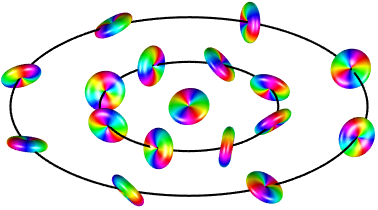
\includegraphics[width=\textwidth]
        {gfx/ch-spin2/C-FM=2_coreless_FM_init_spherical.pdf}
        \caption{\label{subfig: coreless-initial}}
    \end{subfigure}
    \begin{subfigure}{0.45\textwidth}
        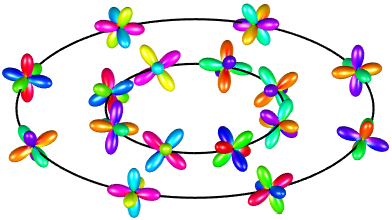
\includegraphics[width=\textwidth]
        {gfx/ch-spin2/C-FM=2_coreless_cyclic_init_spherical.pdf}
        \caption{\label{subfig: DQV-initial}}
    \end{subfigure}
    \caption{\label{fig: coreless-doubly-quantised} Spherical harmonic
        representation of the vortex configurations on each side of the FM-BN
        interface defined in Eq.~\eqref{eq: FM-BN-coreless-DQV}.
        (a): Spin-2 FM coreless vortex given by Eq.~\eqref{eq: FM-BN-coreless}.
        (b): Doubly quantised vortex on the BN side of the interface, given by
        Eq.~\eqref{eq: FM-BN-DQV}.
        \textcolor{red}{Current DQV is for cyclic case, update to BN.}}
\end{figure}
By tracing a point about the vortex line, the phase changes by a total of
\(4\pi \) indicating a doubly quantised vortex.

\subsection{Uniaxial nematic to biaxial nematic}
Consider \(D_1 \neq 0\) and \(D_2 = 0\), then \(\zeta_1 = \zeta_{-1} = 0\).
Furthermore, if \(\tilde{\mu} = \alpha \), then all of \(\zeta_{\pm 2}\) and
\(\zeta_0\) can be non-zero.
\textcolor{red}{Rest of derivation here.}

The final solution reads
\begin{equation}
    \zeta^\mathrm{UN-BN} = \mqty(
    \frac{\sqrt{1 - \eta}}{2} \\
    0 \\
    \sqrt{\frac{1 + \eta}{2}} \\
    0 \\
    \frac{\sqrt{1 - \eta}}{2}
    ),
\end{equation}
where \(\eta = 10q /|c_2|n \in [-1, 1]\).
This solution depends only on the quadratic Zeeman shift, which can alter the
spinor between phases.
When \(q = c_2n / 10\) the system is in the uniaxial nematic phase.
In the opposite limit when \(q = -c_2n/10\) the system is in the biaxial
nematic phase.
This spinor therefore provides interpolating solutions between the uniaxial
nematic and biaxial nematic phases, engineered through manipulation of the
quadratic Zeeman shift.

The energy of the above state reads \(\epsilon = 2q + c_0n/2 - 10q^2/c_2n\).
Comparing this energy with that of the UN phase
\(\epsilon_\mathrm{UN} = (c_0+c_2/5)n/2\) reveals that this interface is stable
for \(|q| \leq |c_2|n/10\).

The consequence of a spatially-dependent \(\eta \) is revealed from the spin
singlet-duo and -trio amplitudes.
Upon substitution of the above equation into \textcolor{red}{Define duo and trio
    amplitudes, more than likely in theory chapter} yields
\begin{equation}
    \begin{aligned}
        |A_{20}|^2 & = \frac{1}{10} \left[(\eta^2-1)\cos\theta
        + \eta^2 + 1\right],                                          \\
        |A_{30}|^2 & = \frac{1+\eta}{4} \left[3\left(\eta ^2-1\right)
            \cos\theta
            + \eta(5 \eta -8) + 5\right],
    \end{aligned}
\end{equation}
where \(\theta = \chi_2 + \chi_{-2} - 2\chi_0\) and \(\chi_j = Arg(\psi_j)\) for
component \(j=-2, 0, 2\).
We plot both the singlet-duo and -trio amplitudes in
Fig.~\ref{fig: UN-BN-duo-trio} in a parameter space of \((\eta, \theta)\).
\begin{figure}
    \centering
    \includegraphics[width=0.75\textwidth]{example-image-a}
    \caption{\label{fig: UN-BN-duo-trio} Contour of singlet-duo and -trio
        amplitude goes here.}
\end{figure}


\subsection{Cyclic to nematic}
The resulting solution reads
\begin{equation}\label{eq: C-N-interpolating-spinor}
    \zeta^\mathrm{C-N} = \mqty(\frac{\sqrt{1 + \eta}}{2} \\ 0 \\
    i\sqrt{\frac{1 - \eta}{2}} \\ 0 \\ \frac{\sqrt{1 + \eta}}{2}),
\end{equation}
where \(\eta = -10q/(c_2n)\).
The quadratic Zeeman shift can be used to interpolate the above solution between
different phases.
At \(q = 0\) the above solution becomes the three component cyclic
\(\zeta_\mathrm{C} = {(1, 0, i\sqrt{2}, 0, 1)}^T/2\).
The sign of the quadratic Zeeman shift determines which nematic state is chosen.
If \(q = -c_2n/10\) then the solution becomes biaxial nematic
\(\zeta_\mathrm{BN} = {(1, 0, 0, 0, 1)}^T/\sqrt{2}\).
In the opposite limit of \(q = c_2n/10\) then the system is in the uniaxial
nematic state \(\zeta_\mathrm{UN} = {(0, 0, 1, 0, 0)}^T\).

\subsection{Cyclic to ferromagnetic}
An additional stationary solution can be found by considering \(D_1=D_2=0\).
Eq.~\eqref{eq: D2} and Eq.~\eqref{eq: D1} can then be solved exactly, to yield
\begin{equation}
    \tilde{\mu} = \pm \sqrt{4q^2 + |\alpha|^2}.
\end{equation}
If \(q \neq 0\), then \(\tilde{\mu} \neq \alpha \) which implies \(\zeta_0=0\)
from Eq.~\eqref{eq: spin-2-stationary-zeta0-recast}.
Zero transverse magnetisation then implies we have
\(0 = 2c_1n(\zeta_2^*\zeta_{1} + \zeta_{-1}^*\zeta_{-2})\).
\textcolor{red}{Rest of derivation here.}

The final solution reads
\begin{equation}
    \zeta^\mathrm{C-FM} = \mqty(\sqrt{\frac{1 + f_z}{3}} \\ 0 \\ 0 \\
    \sqrt{\frac{2 - f_z}{3}} \\ 0),
\end{equation}
where \(f_z = (p - q) / (c_1n)\).
At zero magnetisation, \(f_z = 0\), this solution is precisely the two-component
cyclic state.
The solution also interpolates between different ferromagnetic states depending
on the magnetisation.
If \(f_z = -1\) one recovers an FM-1 solution.
Conversely, \(f_z = 2\) yields the FM-2 solution.
This spinor there provides an interpolating solution between the cyclic and
ferromagnetic phases.

\section{Dynamical stability of interface solutions}

\section{Numerical investigations of defect crossing physics}
\subsection{Uniaxial nematic to biaxial nematic interface}
\subsection{Cyclic to ferromagnetic interface}
\subsection{Cyclic to biaxial nematic interface}
